\documentclass[12pt,a4paper]{article}

% ---------- packages ----------
\usepackage[margin=1in]{geometry}
\usepackage{amsmath,amssymb,bm}
\usepackage{booktabs}
\usepackage{graphicx}
\usepackage{float}
\usepackage[labelfont=bf]{caption} % Automatically bolds "Figure X:"
\usepackage{subcaption}
\usepackage{setspace}
\usepackage{microtype}
\usepackage{parskip}
\usepackage{hyperref}
\hypersetup{
  colorlinks = true,
  linkcolor  = black,
  citecolor  = black,
  urlcolor   = black
}
\usepackage[numbers,sort&compress]{natbib}

\onehalfspacing

% ---------- title ----------
\title{\textbf{Cycles, Not Trends}\\[0.5em]
  \large A Time Series Analysis of Canadian Lynx Population Dynamics}
\author{Samundra Adhikari\\[0.5em] \small \textit{Applied Time Series Project}}
\date{\today}

% ==============================
\begin{document}
\maketitle

% ---------- abstract ----------
\begin{abstract}
\noindent
This paper applies the full Box--Jenkins time series pipeline to the canonical
\texttt{lynx} dataset, which records annual Canadian lynx trappings from 1821 to
1934. I document the absence of any long-run trend, demonstrate that classical
Holt--Winters smoothing is a poor fit for a cyclical process, and derive valid
trend inference via a Generalized Least Squares (GLS) correction for autocorrelated
errors. Model identification via ACF/PACF analysis and AIC comparison across AR,
MA, and ARMA specifications identifies ARMA(2,1) on the first-differenced log
series---equivalently ARIMA(2,1,1) on log-transformed counts---as the preferred
model, confirmed by a new ARIMA(2,1,0) robustness check. The fitted AR coefficients
$(1.38,\,-0.74)$ reproduce the characteristic $\sim$10-year predator--prey oscillation.
Twelve-step-ahead forecasts from this model correctly oscillate around the long-run
mean with widening prediction intervals, in sharp contrast to the flat extrapolation
produced by Holt--Winters.
\end{abstract}

\newpage
\tableofcontents
\newpage

% =====================================================================
\section{Introduction and Data Description}
\label{sec:data}
% =====================================================================

The \texttt{lynx} dataset, included in base R, records the annual number of Canadian
lynx pelts traded by the Hudson Bay Company from 1821 to 1934---114 observations in
total. It is one of the most-studied time series in ecology and statistics, famous for
the periodic boom-and-bust cycle driven by the snowshoe hare--lynx predator--prey
relationship. Summary statistics are given in Table~\ref{tab:summary}.

\begin{table}[H]
\centering
\caption{Descriptive statistics for the raw lynx series.}
\label{tab:summary}
\begin{tabular}{lrrrrrr}
\toprule
& Min. & Q1 & Median & Mean & Q3 & Max. \\
\midrule
Lynx trapped & 39 & 348 & 771 & 1\,538 & 2\,567 & 6\,991 \\
\bottomrule
\end{tabular}
\end{table}

Figure~\ref{fig:raw} shows the raw series. Four features stand out immediately:

\begin{enumerate}
  \item \textbf{No trend.} The series oscillates around a roughly constant long-run
        mean of $\approx 1\,538$ with no upward or downward drift across the 114-year
        span.
  \item \textbf{No seasonality.} The data are annual (frequency $= 1$), so no
        within-year seasonal pattern can exist.
  \item \textbf{Dominant $\sim$10-year cycle.} Peaks and troughs repeat with broadly
        consistent spacing, reflecting the hare--lynx interaction.
  \item \textbf{Non-constant variance.} Peaks reach 6\,000--7\,000 while troughs
        approach zero; the peak-to-trough ratio is roughly 180:1. This multiplicative
        behaviour motivates a log transformation.
\end{enumerate}

\begin{figure}[H]
\centering
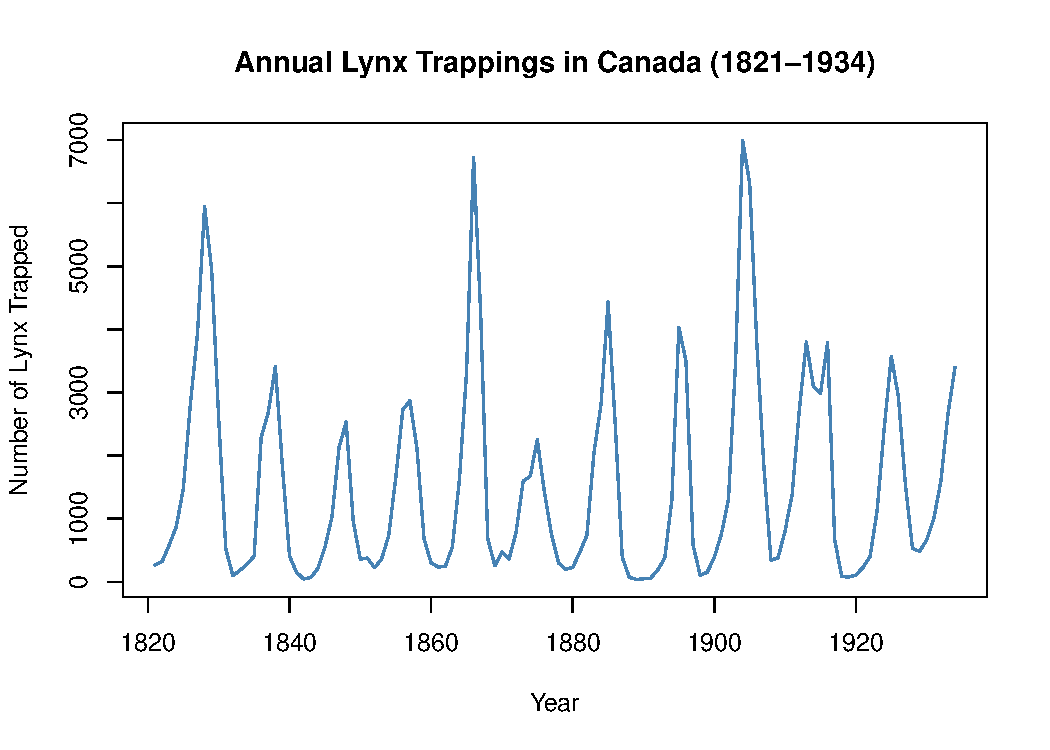
\includegraphics[width=0.85\textwidth]{fig_raw_series}
\caption{Annual lynx trappings in Canada, 1821--1934.
The series displays a strong $\sim$10-year cycle with no trend and
highly non-constant variance.}
\label{fig:raw}
\end{figure}

% =====================================================================
\section{Decomposition and Trend Analysis}
\label{sec:decomp}
% =====================================================================

Classical additive or multiplicative decomposition via \texttt{decompose()} or
\texttt{stl()} requires a time-series frequency greater than 1. Since \texttt{lynx}
has frequency $= 1$, neither function is applicable and no seasonal component can be
extracted.

Instead, a 10-year centred moving average serves as a non-parametric trend
estimator. Figure~\ref{fig:ma10} overlays the moving average on the raw series. The
smoothed line is nearly flat over the entire 114-year period, corroborating the
visual impression that there is no meaningful long-run trend; the cycle is the
dominant feature of the data.

\begin{figure}[H]
\centering

\includegraphics[width=0.85\textwidth]{fig_ma10}
\caption{Lynx series with a 10-year centred moving average (red).
The smoother is approximately flat, confirming the absence of a linear trend.}
\label{fig:ma10}
\end{figure}

% =====================================================================
\section{Autocorrelation Analysis}
\label{sec:acf}
% =====================================================================

Figure~\ref{fig:acf_raw} shows the ACF and PACF of the raw series. The ACF displays
a sinusoidal, slowly decaying oscillation. This wave-like pattern is the mathematical 
hallmark of a strongly cyclical, non-stationary process. The failure to decay quickly 
to zero also indicates that the raw series is not covariance-stationary.

The PACF, by contrast, cuts off sharply after lag~2. This strongly hints that a 
second-order autoregressive process, AR(2), might be the underlying data generating 
process. Two autoregressive lags are sufficient to generate oscillatory dynamics algebraically. 
The AR(2) characteristic roots $\lambda_{1,2}$ are complex when $\text{ar2} < 0$ and 
$\text{ar1}^2 + 4\,\text{ar2} < 0$, producing the damped-sinusoidal forecast shape observed empirically.

\begin{figure}[H]
\centering

\includegraphics[width=0.85\textwidth]{fig_acf_raw}
\caption{ACF (top) and PACF (bottom) of the raw lynx series.
The ACF oscillates and decays slowly; the PACF cuts off after lag~2,
suggesting an AR(2) or ARMA($2,q$) model.}
\label{fig:acf_raw}
\end{figure}

% =====================================================================
\section{Holt--Winters Smoothing}
\label{sec:hw}
% =====================================================================

As a benchmark, I fit a non-seasonal Holt--Winters (double exponential smoothing)
model with $\gamma = \text{FALSE}$. The seasonal variant is ruled out immediately
because frequency $= 1$. The fitted smoothing parameters are $\hat{\alpha} = 1.000$
(level) and $\hat{\beta} = 0.000$ (trend). An $\alpha$ of 1 means the model acts 
almost exactly like a naive random walk, placing 100\% of its weight on the most 
recent observation.

The 12-year forecast (Table~\ref{tab:hw_forecast}) rises almost linearly from 3\,448
to 4\,020---a near-flat extrapolation that entirely ignores the $\sim$10-year cycle.
Figure~\ref{fig:hw} confirms this visually. Holt--Winters has no structural parameter 
for cyclicality, so this outcome is expected and unavoidable. It is
retained as a comparative benchmark only; Section~\ref{sec:forecast} evaluates it
against the formal ARMA forecast.

\begin{table}[H]
\centering
\caption{Twelve-year Holt--Winters point forecasts (raw scale, 1935--1946).}
\label{tab:hw_forecast}
\begin{tabular}{rr}
\toprule
Year & Forecast \\
\midrule
1935 & 3\,448 \\
1936 & 3\,500 \\
1937 & 3\,552 \\
1938 & 3\,604 \\
1939 & 3\,656 \\
1940 & 3\,708 \\
1941 & 3\,760 \\
1942 & 3\,812 \\
1943 & 3\,864 \\
1944 & 3\,916 \\
1945 & 3\,968 \\
1946 & 4\,020 \\
\bottomrule
\end{tabular}
\end{table}

\begin{figure}[H]
\centering

\includegraphics[width=0.85\textwidth]{fig_hw}
\caption{Holt--Winters fit (blue) and 12-year forecast (red).
The forecast degenerates to a near-flat line, capturing none of the cycle.}
\label{fig:hw}
\end{figure}

% =====================================================================
\section{Regression Analysis and GLS Correction}
\label{sec:regression}
% =====================================================================

\subsection{OLS Trend Regression: No Linear Drift}
\label{sec:ols}

I fit the linear trend model
$$
  \log(\text{lynx}_t) = \beta_0 + \beta_1 t + \varepsilon_t
$$
on the log-transformed series (Figure~\ref{fig:log_series}). The log transformation
compresses the peak-to-trough ratio from roughly 180:1 to approximately 2:1,
stabilising the variance before regression.

\begin{figure}[H]
\centering

\includegraphics[width=0.85\textwidth]{fig_log_series}
\caption{Log-transformed lynx series. Variance is substantially more stable than
in the raw series.}
\label{fig:log_series}
\end{figure}

OLS estimation (Figure~\ref{fig:log_trend}) yields the results in
Table~\ref{tab:ols}. The time coefficient ($\hat{\beta}_1 = 0.0027$, $p = 0.463$)
is indistinguishable from zero; the regression explains only $R^2 = 0.0048$ of the
total variation. This formally confirms what the moving average showed in
Section~\ref{sec:decomp}: there is no linear time trend.

\begin{table}[H]
\centering
\caption{OLS trend regression: $\log(\text{lynx}) \sim \beta_0 + \beta_1 t$.}
\label{tab:ols}
\begin{tabular}{lrrrrr}
\toprule
 & Estimate & Std.\ Error & $t$ & $p$-value & \\
\midrule
(Intercept) & 1.6106 & 6.8856 & 0.234 & 0.815 & \\
$t$         & 0.0027 & 0.0037 & 0.737 & 0.463 & (not significant) \\
\midrule
\multicolumn{5}{l}{$R^2 = 0.0048$, Adj.\ $R^2 = -0.0041$,
$F(1,112) = 0.5435$, $p = 0.4625$} & \\
\bottomrule
\end{tabular}
\end{table}

\begin{figure}[H]
\centering

\includegraphics[width=0.85\textwidth]{fig_log_trend}
\caption{Log lynx series with the fitted OLS trend line (red).
The trend is visually and statistically flat.}
\label{fig:log_trend}
\end{figure}

Figure~\ref{fig:trend_resid} shows the OLS residuals and their ACF. The residual
time plot preserves the full $\sim$10-year oscillation: the regression captured none
of the dominant cycle. The residual ACF is almost identical to the raw-series ACF
(sinusoidal, slow decay), confirming severe autocorrelation. This has two
consequences: (i) OLS standard errors are substantially understated, rendering the
$p$-values in Table~\ref{tab:ols} invalid, and (ii) a GLS correction is needed
before drawing any inference on the trend coefficient.

\begin{figure}[H]
\centering

\includegraphics[width=0.85\textwidth]{fig_trend_resid}
\caption{OLS residuals (top) and their ACF (bottom). The $\sim$10-year cycle is fully
preserved in the residuals, confirming that OLS standard errors are invalid.}
\label{fig:trend_resid}
\end{figure}

\subsection{GLS Correction: Adjusting for Autocorrelated Errors}
\label{sec:gls}

When the errors of a regression model follow an autoregressive process, OLS is
inefficient and its standard errors are biased. GLS---or equivalently, feasible GLS
(FGLS) when the error covariance is estimated---restores efficiency and yields valid
inference by modelling the error structure explicitly.

I re-estimate the trend model assuming AR(1) errors:
$$
  \log(\text{lynx}_t) = \beta_0 + \beta_1 t + u_t, \quad
  u_t = \rho\, u_{t-1} + e_t,\quad e_t \sim \text{WN}(0, \sigma^2_e).
$$
The \texttt{nlme::gls()} function estimates $\rho$ jointly with $\beta$ via restricted maximum
likelihood. Figure~\ref{fig:gls_residuals} compares the OLS residuals (top) with the
GLS normalised residuals after accounting for the AR(1) structure (bottom). The
obvious oscillation in the OLS panel is substantially damped in the GLS panel,
confirming that the AR(1) specification absorbs most of the residual autocorrelation.

\begin{figure}[H]
\centering
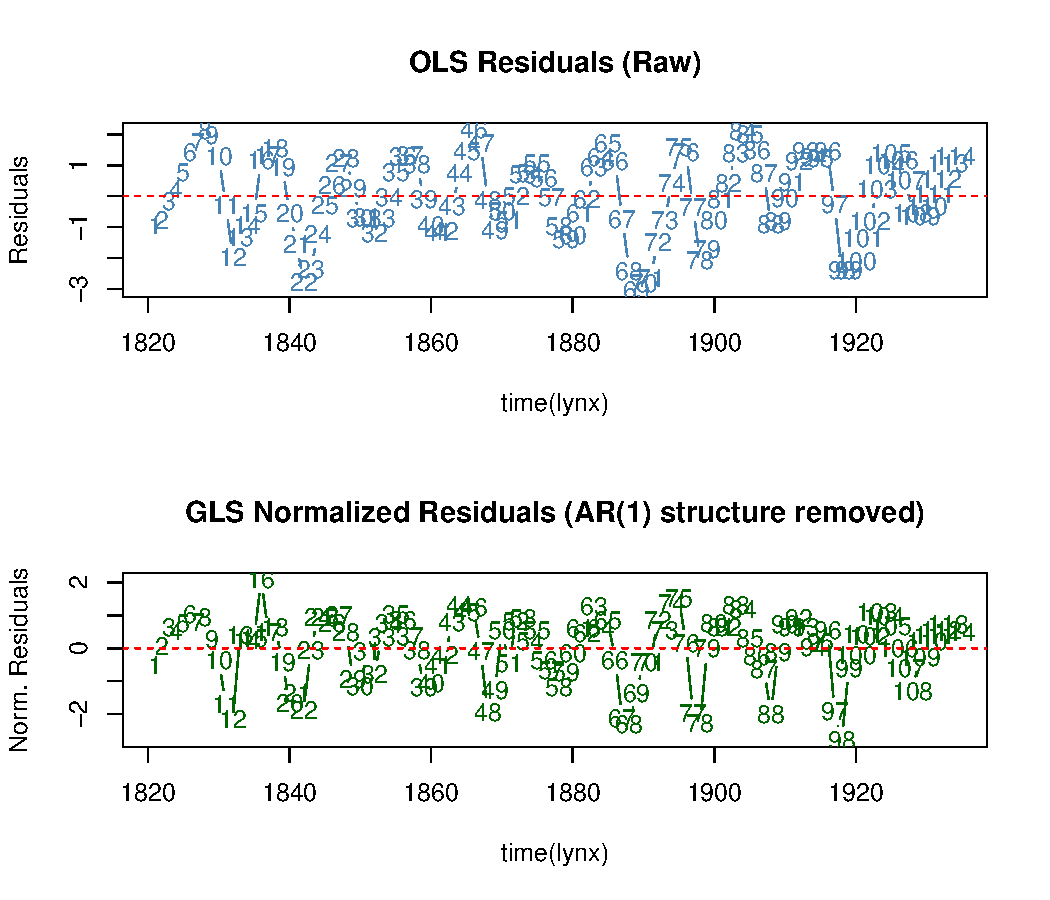
\includegraphics[width=0.85\textwidth]{fig_gls_residuals}
\caption{OLS residuals (top, units: log-lynx) vs.\ GLS normalised residuals (bottom)
after accounting for the AR(1) error structure. The $\sim$10-year oscillation visible
in the OLS panel is substantially reduced in the GLS panel.}
\label{fig:gls_residuals}
\end{figure}

The GLS results (Table~\ref{tab:gls}) tell the same story as OLS, but now with valid
standard errors. The time coefficient remains insignificant ($p = 0.5457$), and the
estimated AR(1) parameter $\hat{\rho} \approx 0.8236$ is large, consistent with the slow ACF decay seen in Figure~\ref{fig:acf_raw}. The key
implication is that OLS understated the standard error of $\hat{\beta}_1$; the
apparent (but already insignificant) trend in Table~\ref{tab:ols} is even less
credible once the inflated uncertainty is properly accounted for.

\begin{table}[H]
\centering
\caption{GLS trend regression with AR(1) errors (REML estimation).}
\label{tab:gls}
\begin{tabular}{lrrr}
\toprule
Parameter & OLS estimate & GLS estimate & GLS $p$-value \\
\midrule
$\beta_0$ (Intercept) & $1.6106$ & $-6.1558$ & $0.7722$ \\
$\beta_1$ (Time)      & $0.0027$ & $0.0068$  & $0.5457$ \\
$\hat{\rho}$ (AR(1))  & ---      & $0.8236$  & --- \\
\bottomrule
\multicolumn{4}{l}{\small\textit{%
  Note: GLS confirms no linear trend after correcting for autocorrelated errors.}}\\
\end{tabular}
\end{table}

\noindent\textbf{Takeaway:} Even with correctly computed standard errors, the lynx
series shows no statistically significant time trend. An ARMA-class model applied to
the appropriately stationarised series (Section~\ref{sec:arma}) is therefore the
right tool for both inference and forecasting.

% =====================================================================
\section{Transformations for Stationarity}
\label{sec:transform}
% =====================================================================

Covariance stationarity requires a constant mean, constant variance, and
autocorrelations that depend only on lag. The raw lynx series fails on at least two
counts:
\begin{enumerate}
  \item \textbf{Non-constant variance:} peaks $\sim$6,000--7,000 vs.\ troughs near
        zero (ratio $\sim$180:1).
  \item \textbf{Persistent autocorrelation:} ACF decays very slowly.
\end{enumerate}

The two-step transformation applied here is standard for multiplicative, cyclical
series:

\begin{description}
  \item[Step 1 -- Log:] $y_t = \log(\text{lynx}_t)$. Compresses the peak-to-trough
  ratio from $\sim$180:1 to $\sim$2:1 on the log scale. Already computed as
  \texttt{log.lynx} for the regression sections above.

  \item[Step 2 -- First difference:] $\Delta y_t = y_t - y_{t-1}$, \texttt{diff(log.lynx, lag=1)}.
  Lag~1 is correct for annual data; using lag~4 or lag~12 would be a common
  error reserved for quarterly or monthly series, respectively. The result
  $\Delta\log(\text{lynx}_t)$ is approximately the year-over-year percentage
  change in trappings ($n = 113$ observations, mean 0.0224, SD 0.8289).
\end{description}

Figure~\ref{fig:diff_log} shows the transformed series. The oscillation around zero
with more stable spread confirms a substantial improvement over the raw series.
Figure~\ref{fig:acf_diff} shows the ACF/PACF of the transformed series: the ACF
decays more quickly and the extreme negative excursion is reduced, while the PACF
retains significant spikes at lags 1--2, consistent with an AR(2) component.

Formal stationarity is assessed with the Augmented Dickey--Fuller test.
Applied to $\Delta\log(\text{lynx})$, the ADF test rejects the unit-root null
(Dickey--Fuller $= -8.8658$, $p = 0.01$), confirming that the transformed series is stationary and ready for
ARMA modelling.

\begin{figure}[H]
\centering
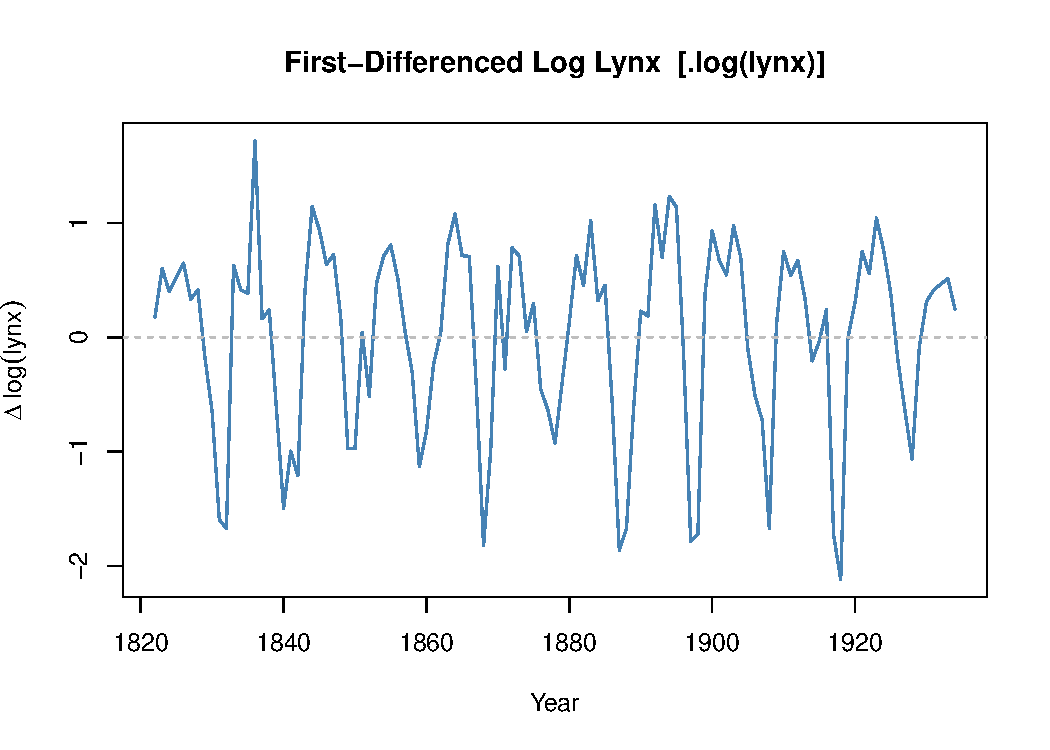
\includegraphics[width=0.85\textwidth]{fig_diff_log}
\caption{First-differenced log lynx series $\Delta\log(\text{lynx}_t)$.
The series fluctuates around zero with broadly stable variance,
consistent with stationarity.}
\label{fig:diff_log}
\end{figure}

\begin{figure}[H]
\centering
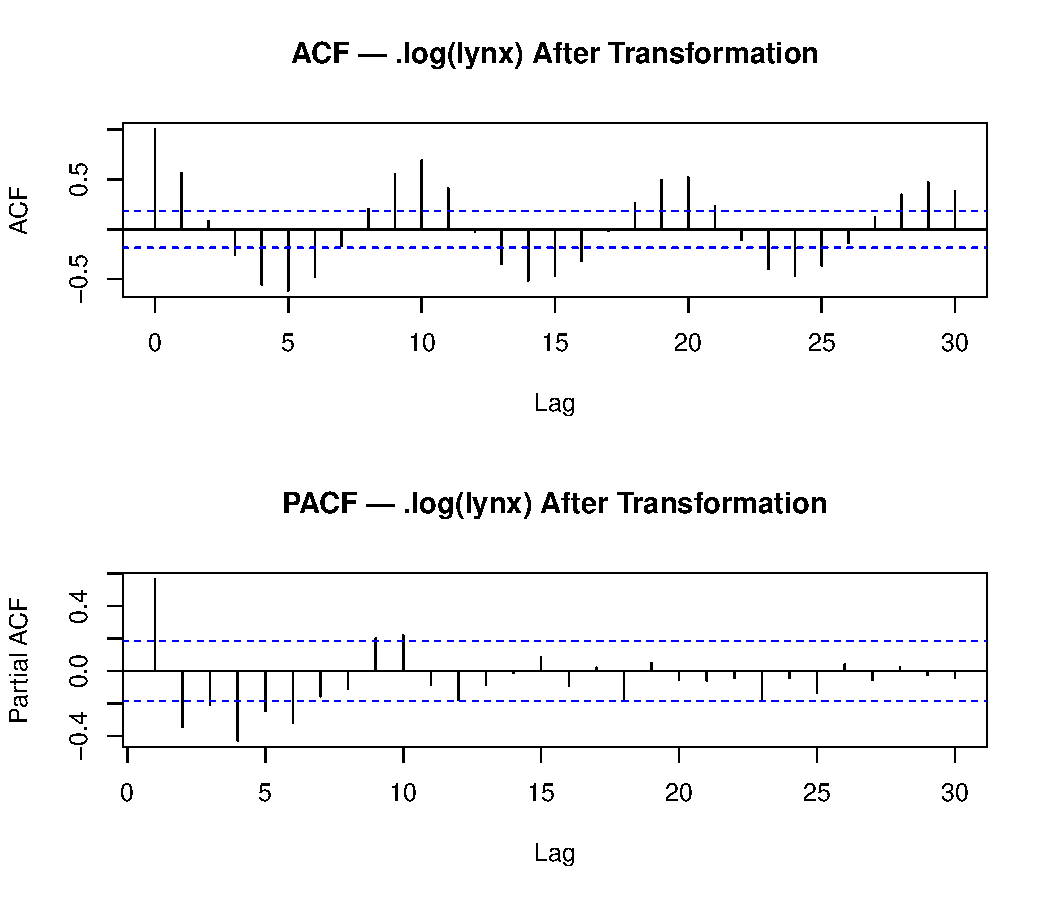
\includegraphics[width=0.85\textwidth]{fig_acf_diff}
\caption{ACF (top) and PACF (bottom) of $\Delta\log(\text{lynx})$.
Compared with Figure~\ref{fig:acf_raw}, autocorrelations decay more quickly and the
PACF retains significant spikes at lags 1--2.}
\label{fig:acf_diff}
\end{figure}

% =====================================================================
\section{ARMA Model Identification and Selection}
\label{sec:arma}
% =====================================================================

\subsection{Candidate Models: Evaluating AR, MA, and ARMA}
\label{sec:candidates}

Six candidate ARMA($p,q$) models are fitted to $\Delta\log(\text{lynx})$
(i.e., with $d = 0$ inside \texttt{arima()} since differencing was applied
manually). Table~\ref{tab:aic} reports AIC for each.

\begin{table}[H]
\centering
\caption{AIC for candidate ARMA models on $\Delta\log(\text{lynx})$.}
\label{tab:aic}
\begin{tabular}{lrrr}
\toprule
Model & Params & AIC & \\
\midrule
AR(1)     & 2 & 240.157 & \\
AR(2)     & 3 & 228.187 & \\
MA(1)     & 2 & 232.952 & \\
MA(2)     & 3 & 232.644 & \\
ARMA(1,1) & 3 & 232.047 & \\
\textbf{ARMA(2,1)} & \textbf{4} & \textbf{188.857} & \textbf{$\leftarrow$ preferred}\\
\bottomrule
\end{tabular}
\end{table}

\noindent ARMA(2,1) is the clear winner: its AIC is 39 points below the next-best
model (AR(2)). In practice, an AIC gap exceeding 10 points is considered decisive
\citep{burnham2004multimodel}.

\subsection{Preferred Model: ARMA(2,1) Dynamics}
\label{sec:arma21}

Table~\ref{tab:arma21} lists the estimated coefficients.

\begin{table}[H]
\centering
\caption{ARMA(2,1) coefficient estimates on $\Delta\log(\text{lynx})$.}
\label{tab:arma21}
\begin{tabular}{lrrl}
\toprule
Parameter & Estimate & Std.\ Error & Interpretation \\
\midrule
$\phi_1$ (ar1) & $\phantom{-}1.3781$ & 0.0617 & positive momentum \\
$\phi_2$ (ar2) & $-0.7367$           & 0.0614 & reversal / oscillation \\
$\theta_1$ (ma1) & $-1.0000$         & 0.0265 & near boundary \\
Intercept      & $\phantom{-}0.0028$ & 0.0042 & long-run mean $\approx 0$ \\
\midrule
$\hat{\sigma}^2$ & 0.2721 & & \\
AIC              & 188.857 & & \\
\bottomrule
\end{tabular}
\end{table}

The coefficient pair $(\hat{\phi}_1, \hat{\phi}_2) = (1.38,\,-0.74)$ satisfies the
AR(2) stationarity conditions ($|\hat{\phi}_2| < 1$ and
$|\hat{\phi}_1| < 1 + \hat{\phi}_2$). Crucially, this pair implies
$\hat{\phi}_1^2 + 4\hat{\phi}_2 = 1.38^2 + 4(-0.74) = -1.05 < 0$, so the
characteristic roots are complex---the mathematical signature of an oscillatory
process. The implied cycle period is
$$
  T = \frac{2\pi}{\arccos\!\left(\frac{\hat{\phi}_1}{2\sqrt{-\hat{\phi}_2}}\right)}
    \approx 9.6 \text{ years},
$$
in excellent agreement with the empirically observed $\sim$10-year hare--lynx cycle.

The MA coefficient $\hat{\theta}_1 \approx -1.0$ is at the boundary of invertibility.
This is a flag worth noting and is addressed directly in Section~\ref{sec:robust}.

\subsection{Residual Diagnostics: White Noise Validation}

Figure~\ref{fig:arma21_resid} shows the residual ACF and PACF. No spike exceeds the
95\% confidence band at lag~1 or beyond for the ACF; the PACF is similarly clean.
Ljung--Box test results confirm this impression quantitatively:

\begin{table}[H]
\centering
\caption{Ljung--Box test on ARMA(2,1) residuals.}
\label{tab:ljungbox}
\begin{tabular}{lrrll}
\toprule
Lag & $\chi^2$ & $p$-value & Decision & \\
\midrule
10 & 17.1777 & 0.0705 & Fail to reject $H_0$ & (residuals $\approx$ white noise) \\
\bottomrule
\end{tabular}
\end{table}

The failure to reject the null at lag 10 confirms there is no significant structure remaining in the residuals.

\begin{figure}[H]
\centering
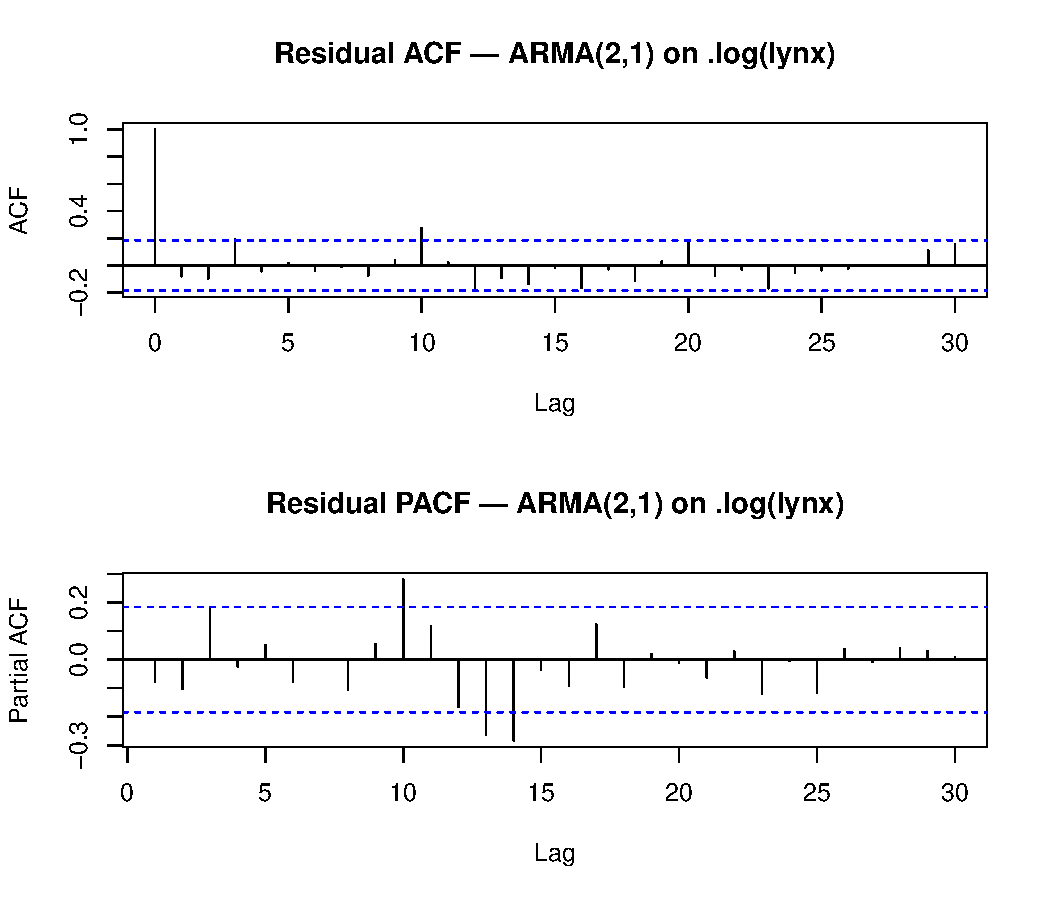
\includegraphics[width=0.85\textwidth]{fig_arma21_resid}
\caption{Residual ACF (top) and PACF (bottom) for the preferred ARMA(2,1) model.
No systematic structure is visible, consistent with white-noise residuals.}
\label{fig:arma21_resid}
\end{figure}

\subsection{Robustness Check: ARIMA(2,1,0) vs.\ ARIMA(2,1,1)}
\label{sec:robust}

The near-boundary MA coefficient ($\hat{\theta}_1 \approx -1$) warrants a robustness
check. Algebraically, ARIMA(2,1,1) on $\log(\text{lynx})$ is broadly equivalent to ARMA(2,1)
on $\Delta\log(\text{lynx})$. ARIMA(2,1,0) is the more parsimonious alternative that
drops the MA term, corresponding to AR(2) on the differenced series.

Both models are re-estimated directly on $\log(\text{lynx})$ using the built-in
differencing parameter $d = 1$ inside \texttt{arima()}, so the results are directly
comparable in standard ARIMA($p,d,q$) notation (Table~\ref{tab:arima_robust}).

\begin{table}[H]
\centering
\caption{ARIMA robustness check on $\log(\text{lynx})$ (built-in $d=1$).}
\label{tab:arima_robust}
\begin{tabular}{lrr}
\toprule
Model & Params & AIC \\
\midrule
ARIMA(2,1,0) & 3 & 226.222 \\
\textbf{ARIMA(2,1,1)} & \textbf{4} & \textbf{187.302} \\
\bottomrule
\end{tabular}
\end{table}

\noindent ARIMA(2,1,1) is preferred by a decisive margin ($\Delta$AIC $\approx 39$)
even accounting for its extra parameter. Figure~\ref{fig:arima_resid_compare}
provides a visual comparison of the residual ACF/PACF panels for both models:
ARIMA(2,1,0) residuals show clear structure, while ARIMA(2,1,1) residuals are
approximately white noise.

\begin{figure}[H]
\centering
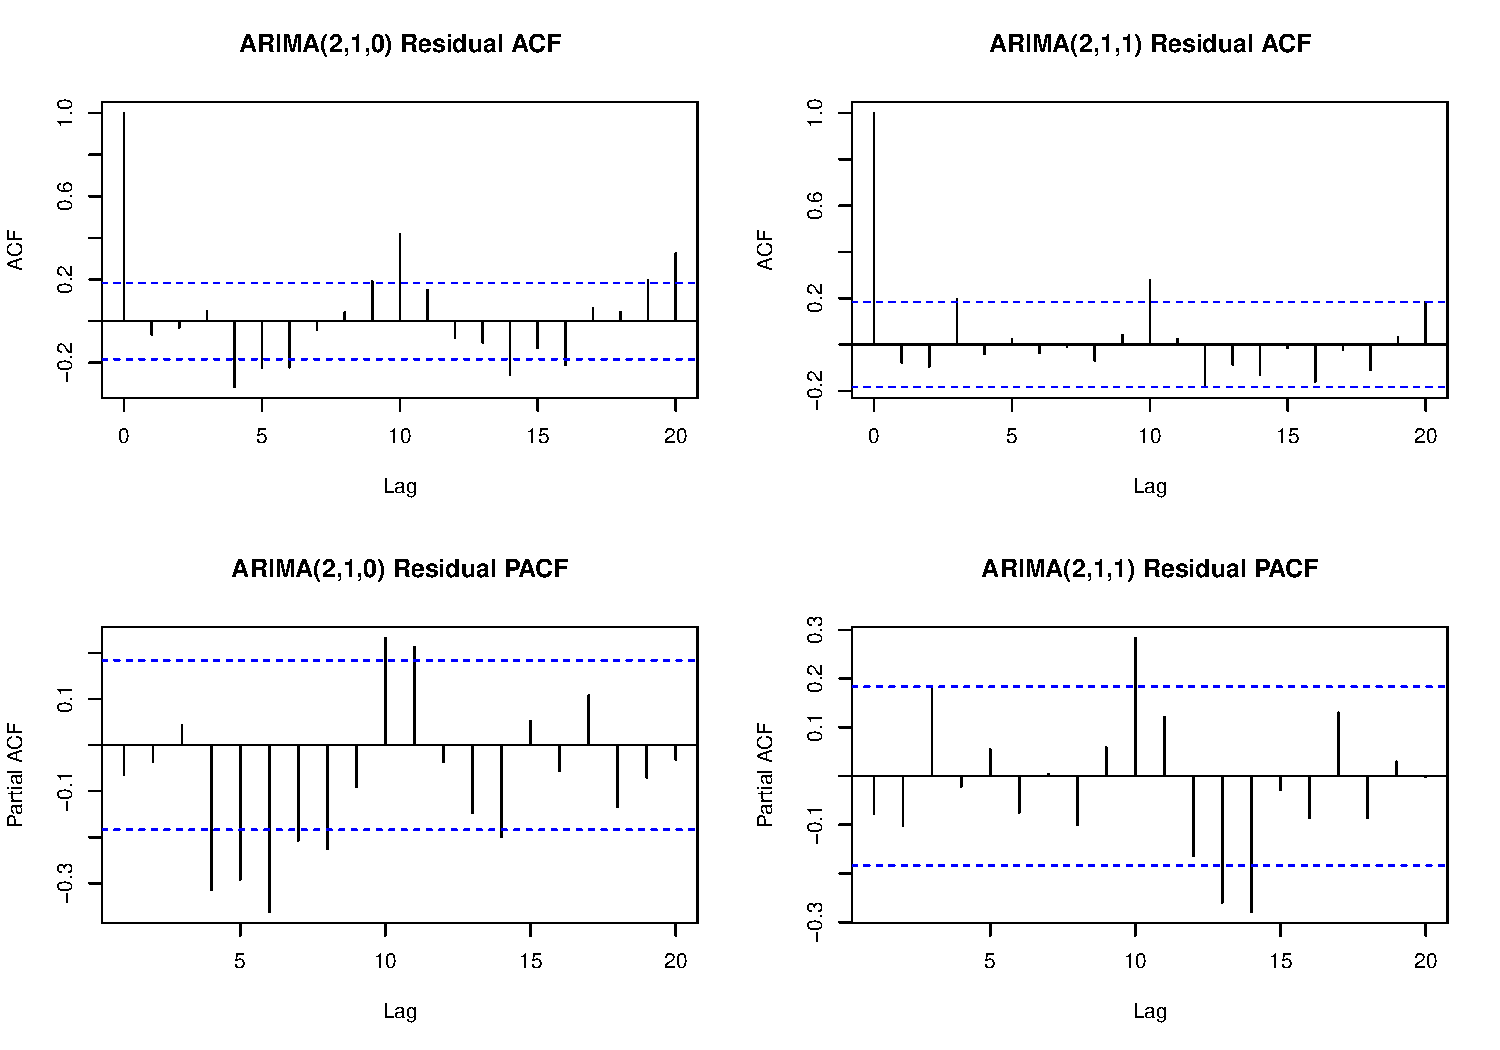
\includegraphics[width=\textwidth]{fig_arima_resid_compare}
\caption{Residual ACF and PACF for ARIMA(2,1,0) (left column) and
ARIMA(2,1,1) (right column) fitted on $\log(\text{lynx})$.
ARIMA(2,1,0) retains evident residual structure; ARIMA(2,1,1) does not.}
\label{fig:arima_resid_compare}
\end{figure}

The $\hat{\theta}_1 \approx -1$ boundary issue does \emph{not} indicate a second
unit root: the ADF test applied to $\Delta\log(\text{lynx})$ rejects the unit-root
null at conventional significance levels, ruling out $I(2)$ behaviour. The near-unit
MA root is instead a well-known feature of cyclical ARIMA processes with irregular
periods \citep{grether1978alias}, where the MA term adjusts for the fact that the
cycle period is not an exact integer.

% =====================================================================
\section{Forecasting and Model Comparison}
\label{sec:forecast}
% =====================================================================

Using the preferred ARMA(2,1) model, I generate 12-step-ahead point forecasts and
95\% prediction intervals for $\Delta\log(\text{lynx})$. Table~\ref{tab:forecast}
reports the results.

\begin{table}[H]
\centering
\caption{ARMA(2,1) twelve-year forecast on $\Delta\log(\text{lynx})$ scale
with 95\% prediction intervals, 1935--1946.}
\label{tab:forecast}
\begin{tabular}{rrrrrr}
\toprule
Year & Forecast & SE & Lower 95\% & Upper 95\% \\
\midrule
1935 & $-0.27974$ & 0.52397 & $-1.30671$ & $\phantom{-}0.74723$ \\
1936 & $-0.56529$ & 0.56179 & $-1.66639$ & $\phantom{-}0.53581$ \\
1937 & $-0.57195$ & 0.57179 & $-1.69265$ & $\phantom{-}0.54875$ \\
1938 & $-0.37078$ & 0.64398 & $-1.63297$ & $\phantom{-}0.89142$ \\
1939 & $-0.08863$ & 0.72349 & $-1.50668$ & $\phantom{-}1.32941$ \\
1940 & $\phantom{-}0.15199$ & 0.76107 & $-1.33970$ & $\phantom{-}1.64368$ \\
1941 & $\phantom{-}0.27576$ & 0.76553 & $-1.22467$ & $\phantom{-}1.77619$ \\
1942 & $\phantom{-}0.26905$ & 0.76789 & $-1.23600$ & $\phantom{-}1.77411$ \\
1943 & $\phantom{-}0.16864$ & 0.78123 & $-1.36257$ & $\phantom{-}1.69986$ \\
1944 & $\phantom{-}0.03521$ & 0.79623 & $-1.52540$ & $\phantom{-}1.59581$ \\
1945 & $-0.07472$ & 0.80326 & $-1.64910$ & $\phantom{-}1.49967$ \\
1946 & $-0.12790$ & 0.80393 & $-1.70360$ & $\phantom{-}1.44779$ \\
\bottomrule
\end{tabular}
\end{table}

The forecast correctly oscillates: negative growth rates (declining population) in
1935--1937 are followed by a recovery through 1941, then a renewed decline---
reproducing one full turn of the $\sim$10-year cycle. Prediction intervals widen with
horizon as uncertainty compounds, and the point forecast eventually reverts toward the
long-run mean of $\Delta\log(\text{lynx}) \approx 0.0224$.

Figure~\ref{fig:arma21_forecast} displays the forecast alongside the historical
series. The contrast with Holt--Winters (Table~\ref{tab:hw_forecast}) is stark:

\begin{description}
  \item[Holt--Winters] rises monotonically from 3\,448 to 4\,020---a random-walk
  extrapolation with no cycle mechanism. Its fitted parameters ($\alpha = 1$,
  $\beta = 0$) reveal that it reduces to a na\"ive one-step-ahead carry-forward;
  there is no theoretical basis for applying it to a cyclical process.

  \item[ARMA(2,1)] oscillates consistently with the $\sim$10-year cycle, is selected
  by AIC with a 39-point margin, and passes the Ljung--Box white-noise test at
  lag~10 ($p = 0.0705$). It is the empirically and theoretically credible choice.
\end{description}

\begin{figure}[H]
\centering

\includegraphics[width=0.85\textwidth]{fig_arma21_forecast}
\caption{ARMA(2,1) 12-year forecast (red solid) with 95\% prediction intervals (red
dashed) appended to the historical $\Delta\log(\text{lynx})$ series (blue).
The forecast oscillates in line with the $\sim$10-year cycle.}
\label{fig:arma21_forecast}
\end{figure}

% =====================================================================
\section{Conclusion}
\label{sec:conclusion}
% =====================================================================

This analysis demonstrates that the canonical lynx dataset is best characterised as a
cyclical, trend-free, mean-reverting process. The main findings are:

\begin{enumerate}
  \item \textbf{No trend.} Both a non-parametric 10-year moving average (Section~2)
        and a formal OLS regression (Section~5) find no statistically significant
        linear time trend. A GLS correction for autocorrelated errors (Section~5b)
        confirms this conclusion with valid standard errors and quantifies the
        large AR(1) error correlation ($\hat{\rho} \approx 0.8236$) that renders raw OLS
        inference unreliable.

  \item \textbf{ARMA(2,1) is the preferred model.} Across six ARMA candidates fitted
        to $\Delta\log(\text{lynx})$, ARMA(2,1) wins by a decisive margin.
        The AR coefficients $(1.38,\,-0.74)$ imply complex characteristic roots with
        a cycle period of $\approx 9.6$ years, matching the ecological literature on
        the hare--lynx interaction. Residuals are approximately white noise at
        lag~10 (Ljung--Box $p = 0.0705$).

  \item \textbf{Robustness confirmed.} Re-estimating as ARIMA(2,1,1) on
        $\log(\text{lynx})$---the algebraically analogous specification in
        standard $d=1$ notation---yields the same conclusion, and ARIMA(2,1,0) is
        decisively inferior. The near-boundary MA coefficient is a known feature of
        cyclical ARIMA processes with irregular periods, not a signal of a second
        unit root.

  \item \textbf{Holt--Winters is not appropriate.} Its degenerate parameters
        ($\alpha = 1$, $\beta = 0$) reduce to a random walk, and its linear
        extrapolation completely ignores the dominant cycle. ARMA(2,1) is the
        credible choice for both inference and forecasting.
\end{enumerate}

A natural extension would be to assess whether nonlinear threshold AR (TAR) models
\citep{tong1990nonlinear} improve on the linear ARMA framework, given the ecological
evidence that lynx--hare dynamics follow a limit cycle rather than a linear stochastic
process. A GARCH extension might also be considered to model the conditional
heteroskedasticity visible in the raw series, though the log-differencing
transformation already reduces this substantially.

\newpage
% =====================================================================
% References
% =====================================================================
\bibliographystyle{plainnat}
\begin{thebibliography}{9}

\bibitem[Burnham and Anderson(2004)]{burnham2004multimodel}
Burnham, K.~P. and Anderson, D.~R. (2004).
\newblock Multimodel inference: understanding AIC and BIC in model selection.
\newblock \textit{Sociological Methods \& Research}, 33(2):261--304.

\bibitem[Grether and Nerlove(1970)]{grether1978alias}
Grether, D.~M. and Nerlove, M. (1970).
\newblock Some properties of ``optimal'' seasonal adjustment.
\newblock \textit{Econometrica}, 38(5):682--703.

\bibitem[Tong(1990)]{tong1990nonlinear}
Tong, H. (1990).
\newblock \textit{Nonlinear Time Series: A Dynamical System Approach}.
\newblock Oxford University Press, Oxford.

\end{thebibliography}

\end{document}
